% Author	Rajath Shashidhara
% Email		rajath.shashidhara@gmail.com
%
% This work is licensed under the Creative Commons Attribution 4.0 International License. 
% To view a copy of this license, visit http://creativecommons.org/licenses/by/4.0/.

\chapter{Aubry-Andre-Harper Model}\label{ch:aah}
The study of motion of electrons (spinless, non-relativistic) in a periodic 2-dimensional lattice subject to a constant magnetic field perpendicular to the plane of the lattice, or simply the Landau level problem on a lattice, 
has generated a lot of interest due to the fractal nature of the spectrum, presence of a sharp metal-insulator phase transition and its connection to quantum hall effect. We shall 
systematically explore this problem and its close connection to the research work carried out in this thesis.

Several interesting properties of this system are attributed to the competing driving forces in the problem - the cyclotron motion due to the magnetic field and the wave properties of periodic
potential. In the limiting cases, the system maps to Landau problem and free electron motion in a lattice system respectively.

The coordinate axes are oriented such that the periodic lattice lies in the $x$-$y$ plane and the perpendicular magnetic field is $\mathbf{B} = B\hat{\mathbf{z}}$. Further,
the $\hat{\mathbf{x}}$ and $\hat{\mathbf{y}}$ lie along the perpendicular edges of the square lattice unit cell. The magnetic vector potential in Landau gauge is written as $\mathbf{A} = Bx\hat{\mathbf{y}}$. This choice of gauge is for convenience and does not alter the 
results derived in this section. The square lattice is defined by the set of lattice translation vectors $\mathbf{R} = md \hat{\mathbf{x}} + nd\hat{\mathbf{y}}$ such that $m, n \in \mathbb{Z}$.

Hamiltonian in the presence of magnetic field is obtained by replacing $\hat{\mathbf{p}}$ by $\hat{\mathbf{p}} - e\mathbf{A}$.
\begin{equation}
 \hat{H}(x, y) = \frac{1}{2m}(\hat{\mathbf{p}} - e\mathbf{A})^2 + \hat{V}(x,y)
\end{equation}

\section{Magnetic Translation Operators}
In absence of magnetic field, the set of lattice translation operators form an abelian group and they commute with the translationally invariant hamiltonian. This implies that the translation operators 
and the hamiltonian can be simultaneously diagonalized.
\begin{gather}
\hat{H}(\mathbf{r}) = \hat{H}(\mathbf{r} + \mathbf{R}) \nonumber \\
 \hat{T}_{\mathbf{R}}\ket{\psi(\mathbf{r})} = \ket{\psi(\mathbf{r} + \mathbf{R})} \\
 \hat{T}_{\mathbf{R}} = e^{-\frac{i}{\hbar}\mathbf{R}\cdot\hat{\mathbf{p}}} \\
 \hat{T}_{\mathbf{R}_1}\hat{T}_{\mathbf{R}_2} = \hat{T}_{\mathbf{R}_2}\hat{T}_{\mathbf{R}_1} = \hat{T}_{\mathbf{R}_1 + \mathbf{R}_2}
\end{gather}
\begin{align}
 \hat{T}_{\mathbf{R}}\hat{H}(\mathbf{r})\ket{\psi(\mathbf{r})} &= \hat{H}(\mathbf{r} + \mathbf{R})\ket{\psi(\mathbf{r} + \mathbf{R})} \nonumber \\
 &= \hat{H}(\mathbf{r})\ket{\psi(\mathbf{r} + \mathbf{R})} \nonumber \\
 &= \hat{H}(\mathbf{r})\hat{T}_{\mathbf{R}}\ket{\psi({\mathbf{r})}} \nonumber \\
 \hat{T}_{\mathbf{R}}\hat{H}(\mathbf{r}) &= \hat{H}(\mathbf{r})\hat{T}_{\mathbf{R}}
\end{align} The above properties imply that \cite{ashcroft2010solid, snoke2009solid, jain2007composite}
\begin{gather}
 \hat{H}(\mathbf{r})\ket{\psi_{\mathbf{k}}(\mathbf{r})} = E_{\mathbf{k}}\ket{\psi_{\mathbf{k}}(\mathbf{r})} \\
 \hat{T}_{\mathbf{R}}\ket{\psi_{\mathbf{k}}(\mathbf{r})} = e^{i\mathbf{k}\cdot\mathbf{R}}\ket{\psi_{\mathbf{k}}(\mathbf{r})} \\
 \ket{\psi_{\mathbf{k}}(\mathbf{r})} = e^{i\mathbf{k}\cdot\mathbf{r}}\ket{u_{\mathbf{k}}(\mathbf{r})} \text{ such that } \ket{u_{\mathbf{k}}(\mathbf{r})} = \ket{u_{\mathbf{k}}(\mathbf{r} + \mathbf{R})}
\end{gather} This is the essence of \emph{Bloch theorem}. $\mathbf{k}$ is the crystal momentum and it is confined to the limits $k_{x}, k_{y} \in [0, 2\pi/d)$.

However, in the presence of uniform magnetic field, the hamiltonian is no longer translationally invariant, because $\mathbf{A}(\mathbf{r}) \neq \mathbf{A}(\mathbf{r} + \mathbf{R})$.
Therefore, a new set of translation operators called the \emph{Magnetic translation operators} must be defined \cite{zak1964magnetic,brown1964bloch,fischbeck1970theory,bernevig2013topological,jain2007composite,kohmoto1985topological,florek1997local}, that commutes with the new hamiltonian.

As demonstrated in \cite{jain2007composite,kohmoto1985topological}, the consequence of uniform magnetic field is that the vector potential can be expressed as
\begin{equation*}
 \mathbf{A}(\mathbf{r} + \mathbf{R}) = \mathbf{A}(\mathbf{r}) + \bm{\nabla}\mathcal{G}(\mathbf{r}, \mathbf{R})
\end{equation*}
Therefore, the operation of translation operator on the hamiltonian is equivalent to a gauge transformation
\begin{gather}
 \hat{T}_{\mathbf{R}}\left(\frac{1}{2m}(\hat{\mathbf{p}} - e\mathbf{A}(\mathbf{r}))^2\right) = \left(\frac{1}{2m}(\hat{\mathbf{p}} - e\mathbf{A}(\mathbf{r}) - e\bm{\nabla}\mathcal{G}(\mathbf{r}, \mathbf{R}))^2\right)\hat{T}_{\mathbf{R}} \\
 \label{chap_6:magneticgaugetransform}\left(\frac{1}{2m}(\hat{\mathbf{p}} - e\mathbf{A}(\mathbf{r}) - e\bm{\nabla}\mathcal{G}(\mathbf{r}, \mathbf{R}))^2\right) = e^{\frac{ie}{\hbar}\mathcal{G}(\mathbf{r}, \mathbf{R})}\left(\frac{1}{2m}(\hat{\mathbf{p}} - e\mathbf{A}(\mathbf{r}))^2\right)e^{\frac{-ie}{\hbar}\mathcal{G}(\mathbf{r}, \mathbf{R})}
\end{gather}
Now we know that
\begin{equation}
 \hat{\mathcal{T}}_{\mathbf{R}} = e^{\frac{-ie}{\hbar}\mathcal{G}(\mathbf{r}, \mathbf{R})}\hat{T}_{\mathbf{R}}
\end{equation} commutes with $\hat{H}$, and we call them magnetic translation operators.
In Landau gauge, $\bm{\nabla}\mathcal{G}(\mathbf{r}, \mathbf{R}) = BR_{x}\hat{\mathbf{y}}$, which means that $\mathcal{G}(\mathbf{r}, \mathbf{R}) = BR_{x}y$
and $\hat{\mathcal{T}}_{\mathbf{R}} = e^{\frac{-ie}{\hbar}BR_{x}y}\hat{T}_{\mathbf{R}}$.
But, the magnetic translation operators do not form a group. On explicit calculation, one can show that
\begin{equation*}
 \hat{\mathcal{T}}_{\mathbf{R}}\hat{\mathcal{T}}_{\mathbf{R}'} = e^{\frac{-ie}{\hbar}BR_{x}'R_{y}}\hat{\mathcal{T}}_{\mathbf{R} + \mathbf{R}'}
\end{equation*} If $\hat{\mathcal{T}}_{x}$ and $\hat{\mathcal{T}}_{y}$ translate by unit length along $\hat{\mathbf{x}}$ and $\hat{\mathbf{y}}$ respectively, then
\begin{equation*}
 \hat{\mathcal{T}}_{x}\hat{\mathcal{T}}_{y} = e^{i2\pi\frac{e}{h}Bd^2}\hat{\mathcal{T}}_{y}\hat{\mathcal{T}}_{x}
\end{equation*}

If we assume that the magnetic flux through a unit cell is rational
\begin{equation}
 \alpha = \frac{e}{h}Bd^2 = \frac{p}{q} \text{ such that } p,q \in \mathcal{Z}^{+} \text{ and } gcd(p, q) = 1
\end{equation} and define magnetic translation vectors
\begin{equation}
 \mathcal{R} = qmd \hat{\mathbf{x}} + nd \hat{\mathbf{y}} \text{ such that } m,n \in \mathcal{Z}
\end{equation} then, a subset of magnetic translation operators, that translate by units of magnetic unit cell form a group
\begin{equation}
 \hat{\mathcal{T}}_{\mathcal{R}}\hat{\mathcal{T}}_{\mathcal{R}'} = e^{-i2\pi\frac{e}{h}Bm_{1}n_{2}qd^2}\hat{\mathcal{T}}_{\mathcal{R} + \mathcal{R}'} = e^{-i2\pi p m_{1}n_{2}}\hat{\mathcal{T}}_{\mathcal{R} + \mathcal{R}'} = \hat{\mathcal{T}}_{\mathcal{R} + \mathcal{R}'}
\end{equation} When the magnetic flux is irrational it is incommensurate with the periodicity of the lattice. The magnetic translation group can no longer be defined. The case of irrational magnetic flux is studied in \parencite{obermair1976bloch}. Operators in the magnetic translation group commute with each other. Also,
translation by magnetic unit cell $x=qd$ and $y=d$ gives 
\begin{equation}
 \hat{\mathcal{T}}_{\mathrm{qx}}\hat{\mathcal{T}}_{\mathrm{y}} = e^{i2\pi\alpha q}\hat{\mathcal{T}}_{\mathrm{y}}\hat{\mathcal{T}}_{\mathrm{qx}} = e^{i2\pi p}\hat{\mathcal{T}}_{\mathrm{y}}\hat{\mathcal{T}}_{\mathrm{qx}}=\hat{\mathcal{T}}_{\mathrm{y}}\hat{\mathcal{T}}_{\mathrm{qx}}
\end{equation}
Now we have established the required properties to write the eigenvalue equation
\begin{equation}
 \label{chap_6:magtranseig}\hat{\mathcal{T}}_{\mathcal{R}}\ket{\psi_{\mathbf{k}}(\mathbf{r})} = e^{i\mathbf{k}\cdot\mathcal{R}}\ket{\psi_{\mathbf{k}}(\mathbf{r})}
\end{equation} with $\mathbf{k}$ restricted to magnetic brillouin zone $k_{x} \in [0, 2\pi/qd), k_{y} \in [0, 2\pi/d)$. Inspired from bloch theory,
we can write
\begin{equation}
 \ket{\psi_{\mathbf{k}}(\mathbf{r})} = e^{i\mathbf{k}\cdot\mathbf{r}}\ket{u_{\mathbf{k}}(\mathbf{r})}
\end{equation} However, $\ket{u_{\mathbf{k}}(\mathbf{r}+\mathcal{R})} \neq \ket{u_{\mathbf{k}}(\mathbf{r})}$. This relationship can be determined by applying the definition
of magnetic translation operator on Eq. \eqref{chap_6:magtranseig}.
\begin{equation}
 \ket{u_{\mathbf{k}}(\mathbf{r} + \mathcal{R})} = e^{-i2\pi\frac{e}{h}Bqmdy}\ket{u_{\mathbf{k}}(\mathbf{r})}
\end{equation} This is called the \emph{Generalized bloch condition}.

\section{Tight-Binding Hamiltonian}
To write the hamiltonian under the tight-binding approximation, the wavefunction is expanded as a linear combination of a set of localized states \cite{snoke2009solid, ashcroft2010solid}.
In the absence of magnetic field, the wavefunction is written in terms of the wannier states/single atom states as\footnote{With this method, we obtain one band structure of the hamiltonian as  we 
are accounting for contributions from a single state at each lattice site. Two band tight-binding model is described in \cite{butler1968model}}
\begin{equation*}
 \ket{\psi(\mathbf{r})} = \sum_{\mathbf{R}}{a_{\mathbf{R}} \ket{\phi_{\mathbf{R}}(\mathbf{r})}}
\end{equation*} where the wannier states $\ket{\phi_{\mathbf{R}}}$ are localized at their corresponding lattice sites $\mathbf{R}$.
The overlap integral of wannier states localized at different sites is zero.
\begin{equation}
 \braket{\phi_{\mathbf{R}'}|\phi_{\mathbf{R}}} = \delta_{m'm}\delta_{n'n}
\end{equation}
The tight-binding approximation for the zero-magnetic field case is obtained by plugging the above expansion into the eigenvalue equation
\begin{align}
 \left(\frac{1}{2m}\mathbf{p}^2 + \hat{V}(\mathbf{r})\right)\sum_{\mathbf{R}}{a_{\mathbf{R}} \ket{\phi_{\mathbf{R}}(\mathbf{r})}} &= E\sum_{\mathbf{R}}{a_{\mathbf{R}} \ket{\phi_{\mathbf{R}}(\mathbf{r})}} \nonumber\\
 \sum_{m, n}{\hat{H}_{0}a_{m,n}\ket{\phi_{m,n}(\mathbf{r})}} &= \sum_{m, n}{E a_{m,n}\ket{\phi_{m,n}(\mathbf{r})}} \nonumber\\
 \sum_{k, l}{\ket{\phi_{k,l}}\bra{\phi_{k,l}}}\sum_{m, n}{\hat{H}_{0}a_{m,n}\ket{\phi_{m,n}}} &= \sum_{k, l}{\ket{\phi_{k,l}}\bra{\phi_{k,l}}}\sum_{m, n}{E a_{m,n}\ket{\phi_{m,n}}} \nonumber\\
 \text{Switching dummy indices on the left}\nonumber\\
 \sum_{m, n}{\ket{\phi_{m,n}}\bra{\phi_{m,n}}}\sum_{k, l}{\hat{H}_{0}a_{k,l}\ket{\phi_{k,l}}} &= \sum_{k, l}{\ket{\phi_{k,l}}\bra{\phi_{k,l}}}\sum_{m, n}{E a_{m,n}\ket{\phi_{m,n}}} \nonumber \\
 \sum_{m, n, k, l}{a_{k,l}\braket{\phi_{m,n}|\hat{H}_{0}|\phi_{k,l}}\ket{\phi_{m,n}}} &= \sum_{k, l, m, n}{E a_{m,n} \braket{\phi_{k,l}|\phi_{m,n}}\ket{\phi_{m,n}}}\nonumber\\
 \sum_{m, n}\sum_{k, l}{a_{k,l}\braket{\phi_{m,n}|\hat{H}_{0}|\phi_{k,l}}\ket{\phi_{m,n}}} &= \sum_{k, l, m, n}{E a_{m,n} \delta_{k, m} \delta_{l, n} \ket{\phi_{m,n}}}\nonumber\\
 \sum_{m, n}\sum_{k, l}{a_{k,l}\braket{\phi_{m,n}|\hat{H}_{0}|\phi_{k,l}}\ket{\phi_{m,n}}} &= \sum_{m, n}{E a_{m,n} \ket{\phi_{m,n}}}\nonumber\\
 \text{Comparing coefficients of }\ket{\phi_{m,m}} \nonumber \\ 
 \sum_{k, l}{a_{k,l}\braket{\phi_{m,n}|\hat{H}_{0}|\phi_{k,l}}} &= E a_{m,n} \nonumber \\
 \sum_{k\neq m, l\neq n}{a_{k,l}\braket{\phi_{m,n}|\hat{H}_{0}|\phi_{k,l}}} + a_{m,n}\braket{\phi_{m,n}|\hat{H}_{0}|\phi_{m,n}} &= E a_{m,n}
\end{align}
$\braket{\phi_{m,n}|\hat{H}_{0}|\phi_{m,n}}$ is independent of indices $m, n$ due to translation invariance of $\hat{H}_{0}$. This is set to zero, as this is equivalent to shifting
the energy scale. Translational symmetry also means that 
\begin{equation*}
 \braket{\phi_{m,n}|\hat{H}_{0}|\phi_{k,l}} = \braket{\phi_{m-k,n-l}|\hat{H}_{0}|\phi_{0, 0}}
\end{equation*} Using the above properties, the above equation can be written as
\begin{equation*}
 \sum_{k\neq 0, l\neq 0}{a_{m+k,n+l}\braket{\phi_{0,0}|\hat{H}_{0}|\phi_{k,l}}} = E a_{m,n}
\end{equation*} Designating $W_{k, l} = \braket{\phi_{0,0}|\hat{H}_{0}|\phi_{k,l}}$
Tight-binding approximation entails assuming that the wannier functions are well localized and the overlap between far-off wannier states is approximately zero. Therefore, 
only interactions between the nearest neighbors is significant in the summation defined above. We also expect $W_{1, 0} = W_{-1, 0}$ and $W_{0, 1} = W_{0, -1}$ as justified in \parencite{stockmann2006quantum}.
With these assumptions, the tight-binding equation is written as
\begin{equation}
 W_{1,0}(a_{m+1, n} + a_{m-1, n}) + W_{0, 1}(a_{m, n+1} + a_{m, n-1}) = Ea_{m, n}
\end{equation} In matrix form, the hamiltonian is written as
\begin{equation}
\hat{H}_{0} = \sum_{m,n} W_{1,0}\ket{m+1, n}\bra{m, n} + W_{0,1}\ket{m, n+1}\bra{m, n} + h.c.
\end{equation}
This expression is succinctly expressed in terms of the translation operators
\begin{equation}
  \hat{H}_{0} = W_{1,0}\hat{T}_{x} + W_{0,1}\hat{T}_{y} + h.c.
\end{equation}
When the magnetic field is non-zero, the expansion is written as \cite{luttinger1951effect, wannier1962dynamics, stockmann2006quantum,bernevig2013topological}
\begin{align}
  \ket{\psi(\mathbf{r})} = \sum_{\mathbf{R}}{a_{\mathbf{R}} e^{2\pi \frac{ie}{h}\int_{\mathbf{R}}^{\mathbf{r}}{\mathbf{A}\cdot d\mathbf{r}'}}\ket{\phi_{\mathbf{R}}(\mathbf{r})}}
\end{align}
The line integral in the exponent is taken along the straight line path between the two points. We have used a local gauge transformation of the wannier states in the above expansion.
This is equivalent to the choice of gauge in writing the electromagnetic potential \cite{sakurai2011modern,kitel1971introduction,moriyasu1983elementary}. This transformation is done is the same
spirit as the one we did when we defined the magnetic translation operators in Eq. \eqref{chap_6:magneticgaugetransform}. As shown in \parencite{luttinger1951effect},
the following property holds under the approximation of slowly varying magnetic field
\begin{equation}
 \hat{H}e^{2\pi \frac{ie}{h}\int_{\mathbf{R}}^{\mathbf{r}}{\mathbf{A}\cdot d\mathbf{r}'}}\ket{\phi_{\mathbf{R}}} = e^{2\pi \frac{ie}{h}\int_{\mathbf{R}}^{\mathbf{r}}{\mathbf{A}\cdot d\mathbf{r}'}}\hat{H}_{0}\ket{\phi_{\mathbf{R}}}
\end{equation} and for slowly varying magnetic field, the hopping integrals modify as
\begin{equation}
 \braket{\phi_{\mathbf{R}}|e^{-2\pi \frac{ie}{h}\int_{\mathbf{R}}^{\mathbf{r}}{\mathbf{A}\cdot d\mathbf{r}'}}\hat{H}e^{2\pi \frac{ie}{h}\int_{\mathbf{R}'}^{\mathbf{r}}{\mathbf{A}\cdot d\mathbf{r}'}}|\phi_{\mathbf{R}'}} = e^{2\pi \frac{ie}{h}\int_{\mathbf{R}}^{\mathbf{R}'}{\mathbf{A}\cdot d\mathbf{r}'}} \braket{\phi_{\mathbf{R}}|\hat{H}_{0}|\phi_{\mathbf{R}'}}
\end{equation} The above result is known as \emph{Peirels substitution}. Therefore, the tight-binding hamiltonian in the presence of magnetic field is written as \cite{hofstadter1976energy,bernevig2013topological,fischbeck1970theory}
\begin{equation}
 \hat{H} = \sum_{m, n} W_{1,0}e^{2\pi \frac{ie}{h}\int_{md}^{(m+1)d}{\mathbf{A}\cdot d\mathbf{x}}}\ket{m+1, n}\bra{m, n} + W_{0,1}e^{2\pi \frac{ie}{h}\int_{nd}^{(n+1)d}{\mathbf{A}\cdot d\mathbf{y}}}\ket{m, n+1}\bra{m, n} + h.c.
\end{equation}
In Landau gauge
\begin{equation}
 \label{chap_6:harperprev}\hat{H} = \sum_{m, n} W_{1,0}\ket{m+1, n}\bra{m, n} + W_{0,1}e^{2\pi i \alpha m}\ket{m, n+1}\bra{m, n} + h.c.
\end{equation} where $\alpha$ is the magnetic flux through an unit cell
\begin{equation}
 \alpha = \frac{eBd^2}{h}
\end{equation}
In terms of the lattice translation operators as
\begin{align}
 \hat{H} &= W_{1,0}\hat{T}_{x} + W_{0,1}e^{2\pi i \alpha m}\hat{T}_{y} + h.c. \\
 &= W_{1,0}\hat{\mathcal{T}}_{x} + W_{0,1}\hat{\mathcal{T}}_{y} + h.c.
\end{align}
The eigenvalue equation is written as
\begin{equation}
 W_{1,0}(a_{m+1, n} + a_{m-1, n}) + W_{0, 1}(e^{2\pi i \alpha m}a_{m, n+1} + e^{-2\pi i \alpha m}a_{m, n-1}) = Ea_{m, n}
\end{equation}
Coefficients in the above equation, involve only $m$ and do not depend on $n$. We therefore assume plane wave behaviour along y-direction and assume
$a_{mn} = e^{in\theta}a_m$, where $\theta = k_y d$ \cite{hofstadter1976energy,stockmann2006quantum}. This is also clear from the generalized bloch condition derived in the previous section - $\ket{u}$ is periodic 
under translation along the y-axis by a unit cell. On substitution, we obtain the harper equation \cite{harper1955general,harper1955single,hofstadter1976energy,stockmann2006quantum}
\begin{equation}
 a_{m+1} + a_{m-1} + \lambda \cos(2\pi m \alpha + \theta)a_{m} = Ea_{m}
\end{equation}
% \subsection{q-subbands and degeneracy in the spectrum}
The harper equation is a recurrence relation involving coefficients $a_{0}, a_{1}, \dots$. This recurrence relationship is best expressed in terms of a transfer matrix
\begin{equation}
 \left[ \begin{array}{c} a_{m+1} \\ a_{m} \end{array} \right] = \begin{bmatrix} E - \cos(2\pi m \alpha + \theta) & -1 \\ 1 & 0\end{bmatrix} \left[ \begin{array}{c} a_{m} \\ a_{m-1} \end{array} \right] = \mathbf{T}(m)\left[ \begin{array}{c} a_{m} \\ a_{m-1} \end{array} \right]
\end{equation} In terms of the transfer matrix, we can write
\begin{equation}
 \left[ \begin{array}{c} a_{m+1} \\ a_{m} \end{array} \right] = \left(\prod_{j=1}^{m}\mathbf{T}(j)\right)\left[ \begin{array}{c} a_{1} \\ a_{0} \end{array} \right] = \mathbf{Q}^m\left[ \begin{array}{c} a_{1} \\ a_{0} \end{array} \right]
\end{equation} We have not considered the possibility of this recursion blowing up as $m\rightarrow \infty$ i.e., $a_m \rightarrow \infty$ as $m\rightarrow\infty$. This represents an
unphysical situation that must not be allowed. Under the assumption of rationality of $\alpha$, periodicity of $\cos(2\pi m \alpha + \theta)$ implies that \\$\mathbf{T}(q+1) = \mathbf{T}(1)$ and 
$\mathbf{T}(q)\mathbf{T}(q-1)\dots\mathbf{T}(1) = \mathbf{T}(nq)\mathbf{T}(nq-1)\dots\mathbf{T}((n-1)q+1) = \mathbf{Q}^q$. The matrix $\mathbf{Q}^{q}$ is a function of $E$ and $\theta$.
The condition that the coefficients must be bounded translates to a condition on $\mathbf{Q}^{q}$
\begin{equation}
 |tr(\mathbf{Q}^{q})| \leq 4
\end{equation} The trace of $\mathbf{Q}^{q}$ is q-degree polynomial known as the harper polynomial \cite{hofstadter1976energy, butler1968model,satija2016butterfly} and the energy values
that satisfy the above equation occur in $q$ distinct energy bands. Thus, the spectrum of the hamiltonian has $q$-subbands\footnote{This is not true for even values of $q$ as the middle bands touch. This is
described as the ``kiss'' in \parencite{hofstadter1976energy,satija2016butterfly}}. A physical explanation in terms of there being $q$ potential wells inside each magnetic unit cell is conceivable. But, a 
rigorous mathematical explanation is far more satisfying as much of the content presented in this thesis is beyond the reach of intuition.

\section{Hamiltonian in Momentum Space}
Expanding the lattice localized states in terms of states localized in crystal momentum space $\ket{k_x, k_y}$ using fourier transform
\begin{align}
 \ket{m, n} &= \int_{-\pi}^{\pi}\int_{-\pi}^{\pi}\frac{dk_{x}}{2\pi}\frac{dk_{y}}{2\pi}e^{ik_xm+ik_yn}\ket{k_x, k_y} \\
 \bra{m, n} &= \int_{-\pi}^{\pi}\int_{-\pi}^{\pi}\frac{dk_{x}}{2\pi}\frac{dk_{y}}{2\pi}e^{-ik_xm-ik_yn}\bra{k_x, k_y}
\end{align} where $-\pi \leq k_x, k_y < \pi$ and $\ket{k_x + 2\pi a, k_y + 2\pi b} = \ket{k_x, k_y}$ where $a, b \in \mathbb{Z}$.

Consider\footnote{Limits of integration are not written for typesetting convenience}
\begin{align*}
 &W_{1,0} \sum_{m, n} \ket{m+1,n}\bra{m,n} + \ket{m-1,n}\bra{m,n}\nonumber\\ 
 &= \frac{W_{1,0}}{(2\pi)^4}\sum_{m,n}\iiiint dk_{x}dk_{y}dk_{x}'dk_{y}'(e^{ik_x(m+1)+ik_yn}e^{-ik_x'm-ik_y'n} + e^{ik_x(m-1)+ik_yn}e^{-ik_x'm-ik_y'n})\ket{k_x,k_y}\bra{k_{x}',k_{y}'} \nonumber\\
 &= \frac{W_{1,0}}{(2\pi)^4}\iiiint dk_{x}dk_{y}dk_{x}'dk_{y}'\sum_{m,n}(e^{ik_x}e^{i(k_x-k_x')m}e^{i(k_y-k_y')n} + e^{-ik_x}e^{i(k_x-k_x')m}e^{i(k_y-k_y')n})\ket{k_x,k_y}\bra{k_{x}',k_{y}'} \nonumber \\
 &=\frac{W_{1,0}}{(2\pi)^2}\iiiint dk_{x}dk_{y}dk_{x}'dk_{y}'(e^{ik_x}+e^{-ik_x}) \delta(k_x-k_x') \delta(k_y-k_y')\ket{k_x,k_y}\bra{k_{x}',k_{y}'} \nonumber \\
 &= \frac{2W_{1,0}}{(2\pi)^2} \iint dk_{x}dk_{y} \cos(k_x)\ket{k_x,k_y}\bra{k_{x},k_{y}}
\end{align*}
\begin{align*}
 &W_{0,1} \sum_{m, n}\ket{m, n+1}\bra{m, n} e^{i2\pi\alpha m} \\
 &= \frac{W_{1,0}}{(2\pi)^4}\sum_{m,n}\iiiint dk_{x}dk_{y}dk_{x}'dk_{y}'e^{ik_xm+ik_y(n+1)}e^{-ik_x'm-ik_y'n}e^{i2\pi\alpha m}\ket{k_x,k_y}\bra{k_{x}',k_{y}'}\\
 &= \frac{W_{1,0}}{(2\pi)^4}\iiiint dk_{x}dk_{y}dk_{x}'dk_{y}'\sum_{m,n}e^{i(k_x-k_x'+2\pi\alpha)m}e^{i(k_y-k_y')n}e^{ik_y}\ket{k_x,k_y}\bra{k_{x}',k_{y}'}\\
 &= \frac{W_{1,0}}{(2\pi)^2}\iiiint dk_{x}dk_{y}dk_{x}'dk_{y}' e^{ik_y} \delta(k_x+2\pi\alpha-k_x') \delta(k_y-k_y')\ket{k_x,k_y}\bra{k_{x}',k_{y}'}\\
 &= \frac{W_{1,0}}{(2\pi)^2}\iint dk_{x}dk_{y} e^{ik_y}\ket{k_x+2\pi\alpha,k_y}\bra{k_{x},k_{y}}\\
\end{align*}
Similarly,
\begin{equation*}
 W_{0,1} \sum_{m, n}\ket{m, n-1}\bra{m, n} e^{-i2\pi\alpha m} = \frac{W_{1,0}}{(2\pi)^2}\iint dk_{x}dk_{y} e^{-ik_y}\ket{k_x-2\pi\alpha,k_y}\bra{k_{x},k_{y}}
\end{equation*}
The hamiltonian in the momentum space is 
\begin{equation}
 \hat{H} = \int_{-\pi}^{\pi}\int_{-\pi}^{\pi}{\frac{dk_{x}}{2\pi}\frac{dk_{y}}{2\pi} \left[ 2W_{1,0}\cos(k_{x}) \ket{k_x,k_y}\bra{k_{x},k_{y}} + W_{1,0}e^{ik_y}\ket{k_x+2\pi\alpha,k_y}\bra{k_{x},k_{y}} + h.c.\right]}
\end{equation} The hamiltonian has hopping terms mixing $(k_x, k_y)$ with $(k_x + 2\pi\alpha, k_y)$. We can sector the brillouin zone into $q$ zones of $2\pi/q$ size each. This partitioning is
guided by our insight that two wavevectors in the same sector do not mix with each other. This enables us to write the hamiltonian as \cite{bernevig2013topological}
\begin{align}
 H &= \frac{1}{(2\pi)^2}\int_{\frac{-\pi}{q}}^{\frac{\pi}{q}}\int_{-\pi}^{\pi}{dk_{x}^{0}dk_{y} \hat{H}_{k_x^0,k_y}} \\
 \hat{H}_{k_x^0,k_y} = \sum_{n=0}^{q-1} &[-2W_{1,0}\cos(k_{x}^{0} + 2\pi\alpha n)\ket{k_x^{0}+2\pi\alpha,k_y}\bra{k_x^{0}+2\pi\alpha,k_y} \nonumber \\
 &- W_{0,1}(e^{ik_y}\ket{k_x^{0}+2\pi\alpha(n+1),k_y}\bra{k_x^{0}+2\pi\alpha n,k_y} \nonumber \\
 &+ e^{-ik_y}\ket{k_x^{0}+2\pi\alpha(n-1),k_y}\bra{k_x^{0}+2\pi\alpha n,k_y})] 
\end{align} Our new momentum variable $k_{x}^0$ lies in the magnetic brillouin zone $[-\pi/q, \pi/q]$.

We shall expand the q-site hamiltonian $\hat{H}_{k_x^0, k_y}$ as an eigenvalue equation. With $\ket{\psi} = \sum_{n=0}^{q-1}{a_n \ket{k_{x}^0 + 2\pi\alpha n, k_y}}$, the 
eigenvalue equation is
\begin{equation}
2W_{1,0} \cos(k_{x}^0 + 2\pi\alpha n) a_{n} + W_{0,1} (e^{ik_y} a_{n+1} + e^{-ik_y} a_{n-1}) = E_{k_{x}^0, k_y} a_n
\end{equation} with the periodicity condition $a_{n} = a_{n+q}$.
However, the hamiltonian written in this form is not periodic in $k_x^0 , k_y$. We seek this property as it is necessary when calculating topological invariants - called
chern numbers - intimately related to the concept of geometric phase. We make use of a linear transformation, known as the duality transformation \cite{aubry1980analyticity} to obtain such a hamiltonian
\begin{equation}
 a_{n} = \sum_{m=1}^{q} e^{i2\pi\alpha mn} x_{m}
\end{equation} In terms of $x_{m}$ we obtain
\begin{equation}
 2W_{1,0} \cos(k_y + 2\pi\alpha m)x_{m} + W_{0,1}(e^{-ik_{x}^0} x_{m-1} + e^{ik_{x}^0}x_{m+1}) = E_{k_{x}^0, k_y} x_{m}
\end{equation} This transformation has the effect of switching the roles of $k_{x}^0$ and $k_{y}$.
We can push the $k_{x}^0$ dependence to the corners from the upper/lower diagonal terms by $x_m = e^{-ik_{x}^0 m} b_{m}$
\begin{gather}
 2W_{1,0} \cos(k_y + 2\pi\alpha m)e^{-ik_{x}^0 m} b_{m} + W_{0,1}(e^{-ik_{x}^0} e^{-ik_{x}^0 (m-1)} b_{m} + e^{ik_{x}^0}e^{-ik_{x}^0 (m+1)} b_{m}) = E_{k_{x}^0, k_y} e^{-ik_{x}^0 m} b_{m} \nonumber \\
 2W_{1,0} \cos(k_y + 2\pi\alpha m)b_{m} + W_{0,1}(b_{m-1} + b_{m+1}) = E_{k_{x}^0, k_y} b_{m}
\end{gather}
The requirement that $x_{m+q} = x_{m}$ translates to
\begin{align}
 x_{m+q} &= x_{m} \nonumber \\
 e^{-ik_{x}^0 (m+q)} b_{m+q} &= e^{-ik_{x}^0 m} b_{m} \nonumber \\
 b_{m+q} &= e^{ik_{x}^0 q} b_{m}
\end{align}
The above hamiltonian written in matrix form is
\begin{equation}
H_{ij} = 2W_{1,0} \cos(k_y + 2\pi\alpha m) \delta{ij} + W_{0,1} (\delta_{i+1, j} + \delta_{i, j+1}) + W_{0,1}\delta_{i,q}\delta_{j,1} e^{ik_{x}^0 q} + W_{0,1}\delta_{i,1}\delta_{j,q} e^{-ik_{x}^0 q}
\end{equation}
In the above form the hamiltonian satisfies
\begin{align}
 \hat{H}(k_{x}^0, k_y) &= \hat{H}(k_{x}^0 + 2\pi/q, k_y) \\
 \hat{H}(k_{x}^0, k_y) &= \hat{H}(k_{x}^0, k_y+2\pi)
\end{align} The parametric dependence of $\hat{H}$ on $k_x^0 , k_y$ is described by a torus.

\section{Spectrum} The above Hamiltonian is called the Harper model when $\lambda = W_{1,0}/W_{0,1} = 1$. The general model is called the Aubry-Andre model.
When the energy spectrum of the Harper Hamiltonian is plotted against $\alpha$, the famous Hofstadter butterfly is revealed \cite{hofstadter1976energy}. One of the remarkable aspects
of the energy spectrum is that, it splits into $q$ unique subbands for $\alpha=p/q$. This is confounding, because even a slight variation in $\alpha$ causes $q$ to change rapidly.
Infact, the number of real values between any two real numbers is uncountably infinite. As a result, a rich pattern resembling a butterfly is obtained as the plot. Some characterisitics 
displayed by the plot are \cite{hofstadter1976energy,satija2016butterfly,azbel1964energy,macdonald1983landau}
\begin{enumerate}
 \item $\alpha$ and $N+\alpha$ produce the same spectrum. $\alpha$ may be restricted to $[0,1]$ for this reason.
 \item The energy eigenvalues are symmteric with respect to zero. i.e., if $\epsilon \in spectrum(\alpha)$, then $-\epsilon \in spectrum(\alpha)$.
 \item $|\epsilon| \leq 4$. This is a consequence of the boundedness of the wavefunction discussed earlier.
 \item The energy eigenvalues of irrational $\alpha$ is homeomorphic to a cantor set.
 \item The graph has a recursive structure.
\end{enumerate}

\begin{figure}[h]
 \caption{Hofstadter butterfly.}
 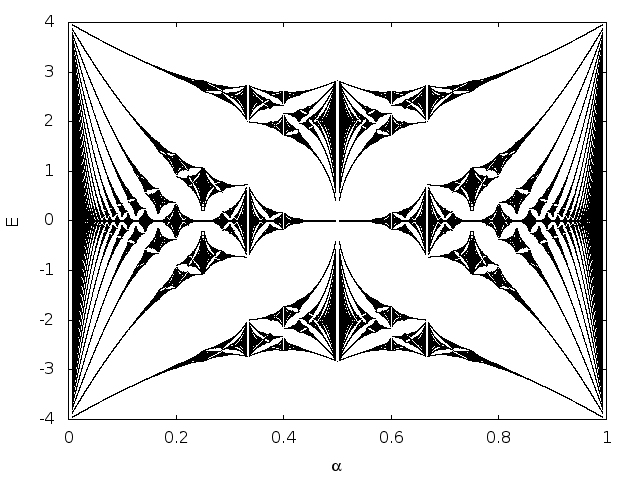
\includegraphics{butterfly}
 \centering
\end{figure}

\section{Metal-Insulator phase transition}
The Aubry-Andre model exhibits a phase transition from localized to delocalized behaviour at $\lambda = 2$ for Diophantine irrational numbers \cite{aulbach2004phase,aubry1980analyticity,jitomirskaya1999metal}. Localization means that the wavefunctions are concentrated at
certain lattice sites. Delocalized wavefunctions are roughly uniformly distributed at all lattice sites. Localized wavefunctions have insulator like properties with no effective
contribution to transport of charge, whereas the delocalized wavefunctions contribute to metallic behaviour. The quantitative measure of localization is called as the Inverse Participation Ratio (IPR).
It is defined as 
\begin{equation}
 IPR = \frac{\sum_{n=1}^{L} |a_{n}|^4} {(\sum_{n=1}^{L} |a_{n}|^2)^2}
\end{equation} where an are the expansion coefficients of the energy eigenstates in a local discrete-site basis and L is the number of lattice sites \cite{mishra2016phase, aulbach2004phase, aubry1980analyticity}.
IPR lies in the range $1$ to $1/L$, where $1$ indicates a perfectly localized state and $1/L$ indicates a perfectly delocalized state.

\begin{figure}[h]
\caption{ The metal-to-insulator transition of the
AAH Hamiltonian for the system’s ground state. Plot (a) shows the
IPR versus V0 or $\lambda$ in real space for L = 144, 1597 and 10 946 (top to
bottom) with $\alpha_0 = (\sqrt(5)-1)/2$ (inverse of golden ratio). The inset shows the variation of D2 with V0 which also
exhibits a transition. Plot (b) exhibits the mirror behavior in the dual
space}
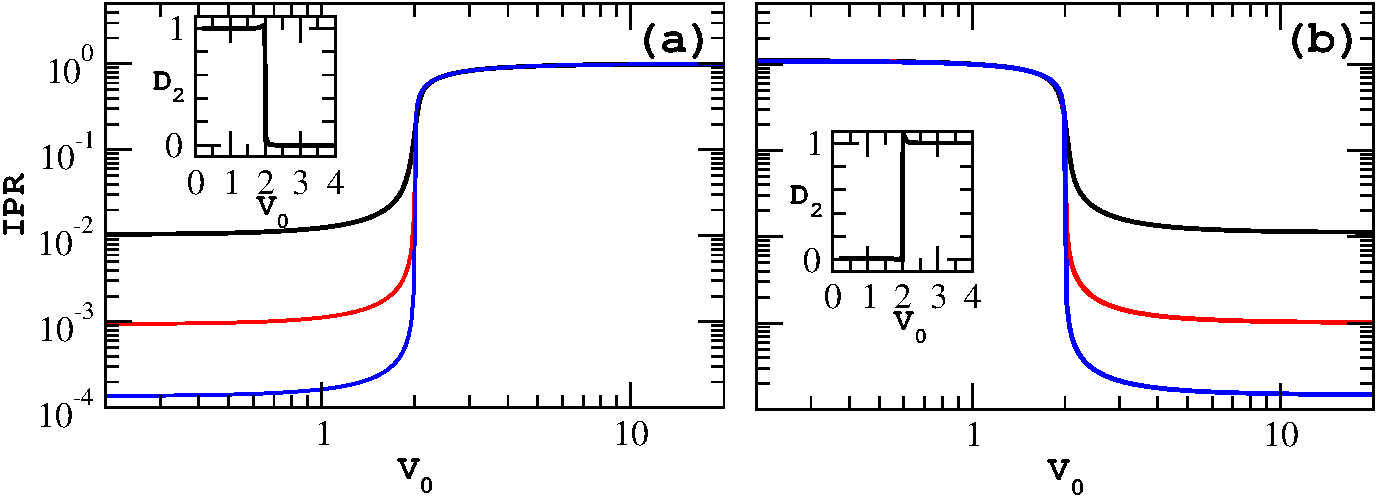
\includegraphics[width=0.75\textwidth]{AA-IPR-D2-Vs-V1byV2}
\centering
\end{figure}
AAH model has a duality transformation of the form \cite{aubry1980analyticity,aulbach2004phase,mishra2016phase}
\begin{equation}
 \ket{m} = \frac{1}{\sqrt{L}}\sum_{n}e^{-i2\pi\alpha_0 m n} \ket{n}
\end{equation} The effect of this transformation is to switch to a momentum space like representation. Wavefunctions localized in real space is delocalized in the dual space and vice versa.
AAH model is an exactly self-dual model i.e., the hamiltonian retains its tri-diagonal form under the duality transformation, and the IPR plot in the dual space is an
exact mirror image of the IPR plot in the real space.
We also seek a relationship between IPR and $L$ of the form $IPR \propto L^{-D_2}$. The sharp transition of $D_2$ to 0 at $V_0 = 2$ indicates that this metal-insulator transition
is independent of length and true even under the limit of $L \rightarrow \infty$.

We shall use the IPR measure to evaluate the metal insulator phase transitions in the variants of the AAH model we study in this thesis.

\section{Hall Conductivity and Chern numbers}
As already mentioned in Chapter \ref{ch:qhe}, the Hall conductivity is a topological invariant. In fact, the harper model was  the first problem for which this result was established \cite{thouless1982quantized}. An interesting
discussion on chern numbers and their physical interpretation as applied to this problem can be found in \parencite{wen1989winding}. Another statement that chern numbers 
are the only topological invariants associated with energy bands is also shown using topological arguments \cite{avron1983homotopy}.
Hall conductivity can be calculated both numerically - using the berry connection, and analytically - using the Streda formula.

Conductivity represents a linear relationship between the current density and the electric field. This is written as
\begin{equation}
 J_{i} = \sum_{j}\sigma_{ij}E_{j}
\end{equation} The off-diagonal term of the conductivity matrix is the hall conductivity.
\begin{equation}
 J_{i} = \sigma_{H}\epsilon_{ij}E_{j}
\end{equation} $\epsilon_{ij}$ is the levi-cevita symbol.
The local charge conservation of electromagnetism is represented by the continuity equation
\begin{equation}
 \mathbf{\nabla}\cdot\mathbf{J} = -\frac{\partial \rho}{\partial t}
\end{equation}
Therefore, for this problem we write
\begin{align}
 \frac{\partial \rho}{\partial t} &= -\mathbf{\nabla}\cdot\mathbf{J} \nonumber \\
 &= -(\partial_{x}J_{x} + \partial_{y}J_{y}) \nonumber \\
 &= -(\partial_{x}(\sigma_{h}E_{y}) + \partial_{y}(-\sigma_{h}E_{x})) \nonumber \\
 &= -\sigma_{H} (\partial_{x}E_{y} - \partial_{y}E_{x}) \nonumber  \\
 \text{Using Maxwell's equation}\\
 &= -\sigma_{H} \frac{\partial B}{\partial t} \nonumber \\
 \text{Therefore} \\
 \sigma_{H} &= \frac{\partial \rho}{\partial B}
\end{align}
This is known as the Streda formula \cite{streda1982quantised, bernevig2013topological}. $\rho$ used in the above equation is the charge density.
If the magnetic flux through an unit cell is a rational number $p/q$, then the charge density can be expressed in terms of
numbers of filled bands (bands below the fermi energy) $r$, as $e\frac{1}{V}\frac{r}{q}$ \cite{kohmoto1992flux,bernevig2013topological}, $V$ is the unit cell area.
Any three integers $p$, $q$ and $r$ can be related by the diophantine equation as
\begin{equation*}
 r = qs_{r} + pt_{r}
\end{equation*} where $s_{r},t_{r} \in \mathbb{Z}$ and $|t_{r}| \leq q/2$, $0\leq r \leq q$.
Implies that
\begin{equation*}
 \frac{r}{q} = s_{r} + \frac{p}{q}t_{r} = s_{r} + \frac{e}{h}BV t_{r}
\end{equation*} Therefore the Hall conductance when fermi level is in the rth gap is \footnote{Admittedly, this proof is not rigorous. Refer to \parencite{streda1982theory} for
a discussion in terms of Landau levels. Also, the TKNN paper also has a different way to arrive at the diophantine equation \cite{thouless1982quantized}.}
\begin{equation*}
 \sigma_{H} = \frac{e^2}{h}t_{r}
\end{equation*}

The Hall conductivity can be calculated numerically by simply performing the integral of the Berry curvature over the Brillouin zone torus. This is conveniently done using
the four-point Bargmann invariant formulation discussed in Chapter \ref{ch:gp}. The validity of this approach for discretized Brillouin zone has been established using 
lattice gauge theory \cite{fukui2005chern,hatsugai2006topological,aidelsburger2016artificial,rasta2016geometry}. The algorithm for the non-abelian case (works even in the presence of degeneracies) is presented step by step below. We intend to calculate chern number
for the $r$th gap.
\begin{enumerate}
 \item Write the Hamiltonian as a periodic function of $k_x$ and $k_y$. This was achieved in the previous section.
 \item Discretize the Brillouin zone. The discrete values of $k_x$ and $k_y$ are given by $k_x[j] = \frac{2\pi}{qN_{x}} j$ where $j=0,1\dots N_{x}-1$ and $k_y[j] = \frac{2\pi}{N_{y}} j$ where $j=0,1\dots N_{y}-1$. Roughly choose $N_{y} \sim qN_{x}$ \footnote{Using Landau gauge. However, this method is applicable for all gauge choices. Suitable modifications are required for symmetric gauge.}. 
 \item For each point on the discrete Brillouin zone, diagonalize the Hamiltonian. $\psi[k,i,j]$ denotes the $k$th eigenvector (eigenvectors ordered in ascending order of corresponding eigenvalues) of
 Hamiltonian at $k_x[i]$ and $k_y[j]$.
 \item For each point $(i,j)$ on the lattice, calculate $r \times r$ matrices $\mathbf{U}^{x}$ and $\mathbf{U}^{y}$. $U^{x}_{[a,b]} = \braket{\psi[a,i,j]|\psi[b,(i+1)mod\,N_{x},j]}$ and $U^{y}_[a,b] = \braket{\psi[a,i,j]|\psi[b,i,(j+1)mod\,N_{y}]}$, where $1\leq a,b \leq r$.
 We denote the $U_{x}[i,j] = \det(\mathbf{U}^{x})$ and $U_{y}[i,j] = \det(\mathbf{U}^{y})$.
 \item The four-point Bargmann invariant (equivalently the Berry curvature times the area) is calculated for each point as 
 \begin{equation*}
  F[i,j] = U_{x}[i,j]U_{y}[(i+1)mod\,N_{x},j]U_{x}^{*}[(i+1)mod\,N_{x},(j+1)mod\,N_{y}]U_{y}^{*}[i,(j+1)mod\,N_{y}]
 \end{equation*}
 \item The chern number is then calculated by summing up the berry curvature values $C = \frac{1}{2\pi i}\sum_{i,j}F[i,j]$. 
\end{enumerate}
The chern numbers for the Harper-Hofstadter problem were successfully calculated using this method. Both methods, of course give the same results!

\begin{figure}[h]
 \centering
 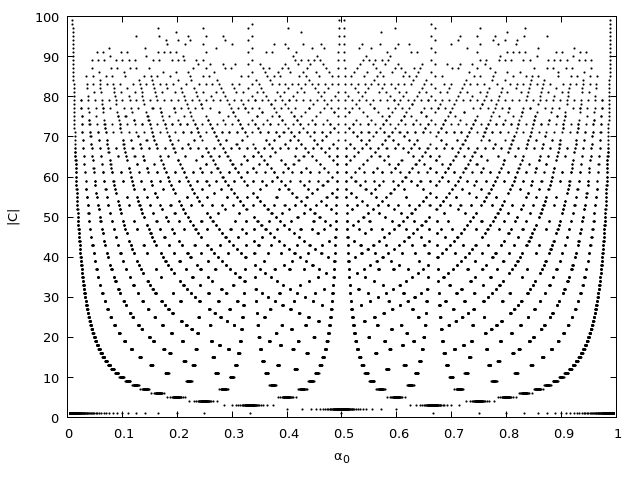
\includegraphics[width=\textwidth]{chern}
 \caption{Absolute value of Chern number $|C|$ of the lowest energy eigenstate as a function of magnetic flux $\alpha_0$.}
\end{figure}
